\chapter{ Технологический раздел}
\label{cha:technological}

    В данном разделе будут выбраны средства реализации ПО и представлен листинг кода. 

    \section{Средства реализации}
        В данной работе используется язык программирования python \cite{python}, так как
        он позволяет написать программу в относительно малый срок.
        В качестве среды разработки использовалась Visual Studio Code \cite{visual-studio-code}. 

        Для замера процессорного времени была использована функция process\_time модуля time \cite{process_time}. 
        Она возвращает значение в долях секунды суммы системного и пользовательского процессорного времени текущего процесса и 
        не включает время, прошедшее во время сна.

    \section{Листинг программы}
        Ниже представлены листинги кода алгоритмов:
        \begin{enumerate}
            \item полным перебором (листинг \ref{lst:brute-force});
            \item бинарным поиском (листинг \ref{lst:binary});
            \item поиском по сегментам (листинг \ref{lst:segment}).
        \end{enumerate}
        
        \begin{lstlisting}[language=python, label=lst:brute-force, caption=Реализация алгоритма поиска слов в словаре полным перебором]

        \end{lstlisting}

        \begin{lstlisting}[language=python, label=lst:binary, caption=Реализация алгоритма двоичного поиска слова в словаре]

        \end{lstlisting}

        \begin{lstlisting}[language=python, label=lst:segment, caption=Реализация алгоритма поиска слова в словаре по сегментам]
        \end{lstlisting}
    
        
    \section{Тестирование}
        В таблице \ref{table:testing} отображён возможный набор тестов
        для тестирования методом чёрного ящика, результаты которого, 
        представленные на рисунке \ref{png:testing:result}, подтверждают
        прохождение программы перечисленных тестов.
        
        \begin{figure}[h!]
            \centering
            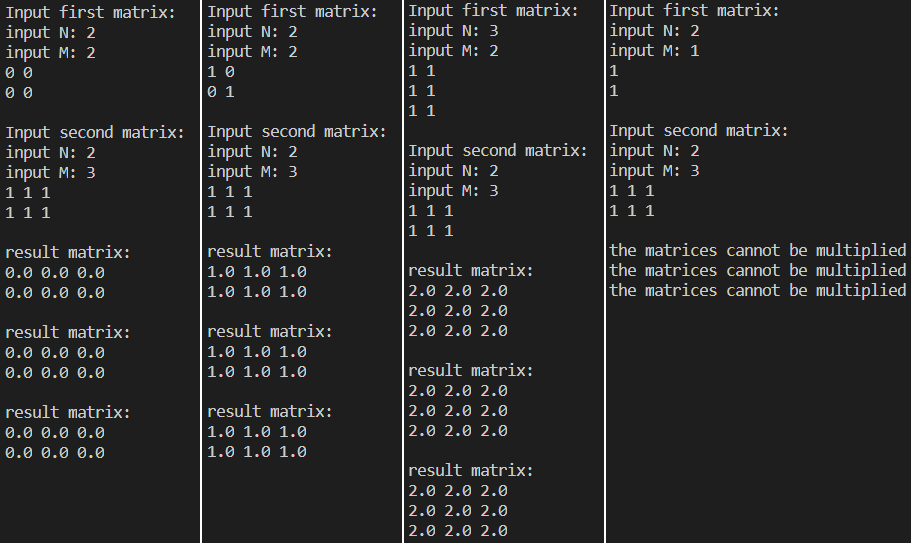
\includegraphics[scale=0.9]{testing.png}
            \caption{Результаты тестирования алгоритмов.}
            \label{png:testing:result}
        \end{figure}
\newpage